\section{Integral Interpolation and the SPH Method}
\label{sec:SPH}

\subsection{Introduction}

In \ac{SPH} an approximate numerical solution is obtained by expressing the continuous media by a set of interpolation points from which to compute the quantities being conserved. These points represent material particles, since the Lagrangian description implies that they move with the flow, 'carrying' a given mass. This perspective into the fundamental idea of the method justifies the \emph{particle} term being applied, in the sense of a numerical mass lump, a macroscopic \emph{quanta} of the discretized medium. 

The method was introduced by \cite{Gingold-1977} and simultaneously by \cite{Lucy-1977}, initially to solve astrophysical problems where Eulerian mesh-based methods were insufficient. As a purely Lagrangian, meshless scheme, \ac{SPH} poses a number of advantages over mesh-based methods. Advection is treated explicitly, since particles carry their properties with them. Motion of the media maps directly as motion of the \ac{SPH} particles. This provides an important advantage for multi-phase problems, as each particle can be assigned to a different phase. Similarly, interfacial or free-surface flows do not require the explicit tracking of the interface or free-surface of interest, as it will be implicitly defined by the positions of the particles. Unlike mesh-based methods, there is no topological connectivity\footnote{Topological connectivity is employed in the context of a numerical discretization exclusively, meaning a fixed list of neighbors with whom to interact does not exist in \ac{SPH}.} between traditional \ac{SPH} particles, as they interact with all of the neighbors according to their radial separation, mediated by an interpolating kernel function. This has profound implications, as many of the issues with generation and evolution of a complex, time-varying mesh are bypassed. Problems involving complex, moving geometry, elastic solids or the fracture of brittle solids are significantly simpler to treat using Lagrangian meshless methods.

Disadvantages of the approach include mostly accuracy and stability concerns, due to their difficult formal description. \ac{SPH} particles are not constrained to stay in a well-ordered, stable configuration. In a regular lattice traditional techniques for stability analysis and convergence studies are well known; in a purely random sampling, as a Monte Carlo method, these qualities are also simple to compute, at least approximately. In \ac{SPH} however, any lattice deforms, not randomly, but according to the conservation equations being solved, introducing an unexpected difficulty in analyzing the method under normal conditions. If on one hand, by respecting the conservation equations, the particles tend to keep evenly spaced, the instantaneous dynamics of the medium can cause the particles to become locally disordered.  \cite{Monaghan-2005} presents an analysis of the interpolation errors that occur for a 1D equi-spaced line of \ac{SPH} particles. \cite{Swegle-1995} and \cite{Morris-1997} performed a stability analysis of \ac{SPH}, providing results for 1D and 2D regular grids of particles. In contrast, there is much less information available on \ac{SPH} errors and instabilities for disordered particles \citep{Ellero-2011}. \cite{Monaghan-2005} and \cite{Dehnen-2012} calculated an upper bound on the errors due to a randomly distributed set of particles, corresponding to a Monte Carlo simulation. Both noted that the distributions resulting from \ac{SPH} simulations are significantly more ordered than pure random positions, hence with higher accuracy than traditional Monte Carlo methods, as \cite{Quinlan-al-2006} explored by attempting to actually derive an error estimate for a generic SPH particle distribution. Even if second order seems to be the limit for traditional \ac{SPH} models \citep{Monaghan-2005, Oger-al-2007}, satisfactory results are achieved due to their inherent conservation properties, that coupled with the other advantages, seem to provide a uniquely useful tool.

%%%%%%%%%%%%%%%%%%%%%%%%%%%%%%%%%%%%%%%%%%%%%%%%%%%%%%%%%%%%%%%%%%%%%%%%%%%%%%%%%%%%%%%%%%
\subsection{Continuous Interpolation}
\label{Subsec:Interpolation}

Consider a scalar field A, expressed as a spatial convolution product with the Dirac Delta function $\delta$

%
\begin{equation} \label{eq:interpolant_1}
A\left( {\ve{r}} \right) = \int_\Omega  {A\left( {{\ve{r}}'} \right)\; \delta \left( {{\ve{r}} - {\ve{r}}'} \right)d{{r}}'},
\end{equation}
%
where $\Omega$ denotes the domain corresponding to the continuous medium. The nature of the Dirac Delta function renders \eqref{eq:interpolant_1} computationally inadequate, forcing its approximation by a suitable weight function $W\left( {{\ve{r}} - {\ve{r}}'} \right)$, called an interpolation kernel, which is a regular function and defines a compact support region\footnote{A function is said to have compact support if it is zero outside of a compact set. In the context of this work, the compact support region is therefore defined as the $\ve{r}$ centered region for which the kernel function $W$ is not zero.}. With $\Omega'$ being the domain centered in $\ve{r}$, one can write

% 
\begin{equation} \label{eq:interpolant_2}
A\left( {\ve{r}} \right) \approx  \left\langle {A} \right\rangle \left( {\ve{r}} \right) = \int_{\Omega '}  {A\left( {\ve{r}'} \right)\; W \left( {{\ve{r}} - {\ve{r}}'} \right)d{{r}}'},
\end{equation}
%
with $\left\langle {A} \right\rangle \left( {\ve{r}} \right)$ defining an interpolated field. Expanding field $A$ as a Taylor series around point $\ve{r}$ and writing $\bar{\ve{r}}=\ve{r}-\ve{r}'$

% 
\begin{equation} \label{eq:interpolant_taylor_1}
A\left( {\ve{r}'} \right) = A\left( {\ve{r}} \right) - \frac{\partial A}{\partial \ve{r}}\cdot \bar{\ve{r}} + \frac{1}{2}\bar{\ve{r}}^T \frac{\partial^2 A}{\partial \ve{r}^T \partial \ve{r}} \bar{\ve{r}} + O\left( |\bar{\ve{r}}|^3 \right)
\end{equation}
%
Replacing \eqref{eq:interpolant_taylor_1} back to \eqref{eq:interpolant_2}
% 
\begin{equation} \label{eq:interpolant_taylor_2}
\begin{split}
\left\langle {A} \right\rangle \left( {\ve{r}} \right) = A\left( {\ve{r}} \right) \int_{\Omega_0} {W \left( {\bar{\ve{r}}} \right)d{{r}}'} - \frac{\partial A}{\partial \ve{r}} \cdot \int_{\Omega_0} {\bar{\ve{r}} W \left( {\bar{\ve{r}}} \right)d{{r}}'} \; + \\ +\; \frac{1}{2} \text{tr}\left(\frac{\partial^2 A}{\partial \ve{r}^T \partial \ve{r}}\right) \cdot \int_{\Omega_0} {\bar{\ve{r}} \times \bar{\ve{r}} W \left( {\bar{\ve{r}}} \right)d{{r}}'} + \int_{\Omega_0} {O\left( |\bar{\ve{r}}|^3 \right) W \left( {\bar{\ve{r}}} \right)d{{r}}'}
\end{split}
\end{equation}
%
where $\Omega_0$ is $\Omega'$ translated to the origin. Noting that in such conditions $d{{r}'}=d\bar{{r}}$, for the approximation $\left\langle {A} \right\rangle \approx A$ to be accurate up to first order, then

% 
\begin{equation} \label{eq:kernel_cond_1}
\int_{\Omega_0} {W \left( \bar{{\ve{r}}} \right)d{{r}}'}=1
\end{equation}
%
and

% 
\begin{equation} \label{eq:kernel_cond_2}
\int_{\Omega_0} {W \left( \bar{{\ve{r}}} \right)\bar{\ve{r}}d{{r}}'}=0
\end{equation}
%

Condition \eqref{eq:kernel_cond_1} implies that the kernel zeroth-order moment should be equal to one, similarly to the Dirac delta distribution. Condition \eqref{eq:kernel_cond_2} asks that the kernel first order moment should be zero. By construction, $\Omega_0$ is centrally symmetric\footnote{A centrally symmetric object in Euclidean space is invariant under point reflection through its center.} and for an even kernel 

% 
\begin{equation} \label{eq:kernel_cond_3}
W \left( -\bar{{\ve{r}}}\right) =W \left( \bar{{\ve{r}}}\right)
\end{equation}
%
and
% 
\begin{equation} \label{eq:kernel_cond_4}
\nabla W \left( -\bar{{\ve{r}}}\right) =-\nabla W \left( \bar{{\ve{r}}}\right)
\end{equation}
%

Making a variable change $\bar{{\ve{r}}}'=-\bar{{\ve{r}}}$, one can write condition \eqref{eq:kernel_cond_2} as

% 
\begin{equation} \label{eq:kernel_cond_5}
\int_{\Omega_0} {W \left( \bar{{\ve{r}}} \right) \bar{\ve{r}} d\bar{\ve{r}}} = \int_{\Omega_0} {W \left( -\bar{{\ve{r}}} \right) \bar{\ve{r}} d\bar{\ve{r}}} = - \int_{\bar{\Omega}_0} {W \left( \bar{{\ve{r}}'} \right) \bar{\ve{r}'} d\bar{\ve{r}}'},
\end{equation}
%
where $\bar{\Omega}_0$ is the symmetric of $\Omega_0$. Assuming symmetrical invariance ($\bar{\Omega}_0 = \Omega_0$), the integral must be equal to its opposite, true only if both integrals are null, rendering condition \eqref{eq:kernel_cond_2} satisfied. We can now reduce \eqref{eq:interpolant_taylor_2} to 

% 
\begin{equation} \label{eq:interpolant_taylor_3}
\left\langle {A} \right\rangle \left( {\ve{r}} \right) = A\left( {\ve{r}} \right) \;+\; O(h^2),
\end{equation}
%
where the integral giving the error is $O(h^2)$ because $W \left( \bar{{\ve{r}}'} \right) \bar{\ve{r}'} d\bar{\ve{r}}' \sim 1/h$. 

Applying approximation \eqref{eq:interpolant_2} to the field $\nabla A$ we may write

% 
\begin{equation} \label{eq:grad_kernel_1}
\begin{split}
\left\langle {\nabla A} \right\rangle \left( {\ve{r}} \right) = \int_{\Omega '} \frac{\partial A \left( {\ve{r}'} \right)}{\partial {\ve{r}}'} \; W \left( \bar{\ve{r}} \right)d{\ve{r}}'\;= \\
=\; \int_{\Omega '} \frac{\partial}{\partial {\ve{r}}'} \left( A \left( {\ve{r}'} \right)\; W \left( \bar{\ve{r}} \right)\right)d{\ve{r}}'\; -\; \int_{\Omega '} A \left( {\ve{r}'} \right) \; \frac{\partial W \left( \bar{\ve{r}} \right)}{\partial {\ve{r}}'}d{\ve{r}}'
\end{split}
\end{equation}
%
It is important to write the identity 

% 
\begin{equation} \label{eq:grad_kernel_2}
\frac{\partial W \left( \bar{\ve{r}} \right)}{\partial {\ve{r}}'}= - \frac{\partial W \left( \bar{\ve{r}} \right)}{\partial {\ve{r}}}
\end{equation}
%
Applying the Gauss theorem to the first integral and the identity to the second yields

% 
\begin{equation} \label{eq:grad_kernel_3}
\left\langle {\nabla A} \right\rangle \left( {\ve{r}} \right) = \oint_{\partial\Omega '} A \left( {\ve{r}'} \right) \; W \left( \bar{\ve{r}} \right) \ve{n}\left( {\ve{r}'} \right) d\Gamma\;+ \; \int_{\Omega '} A \left( {\ve{r}'} \right) \; \frac{\partial W \left( \bar{\ve{r}} \right)}{\partial {\ve{r}}}d{\ve{r}}',
\end{equation}
%
where $\ve{n}\left( {\ve{r}'} \right)$ is the normal unit vector to $\partial\Omega'$. Assuming that the kernel has compact support, the surface integral is reduced to $\partial \Omega \cap \Omega'$ (refer to Figure \ref{fig:cont_kernel}). In an infinite domain, or with a sufficiently distant point $\ve{r}$ from $\partial \Omega$, this boundary integral is zero and Equation \eqref{eq:grad_kernel_3} renders

% 
\begin{equation} \label{eq:grad_kernel_4}
\left\langle {\nabla A} \right\rangle \left( {\ve{r}} \right) = \; \int_{\Omega '} A \left( {\ve{r}'} \right) \; \nabla { W \left( \bar{\ve{r}} \right)}d{\ve{r}}',
\end{equation}
%
This defines a continuously interpolated gradient operator, identical to \eqref{eq:interpolant_2}, but using the kernel gradient as the interpolation function. This is equivalent to writing

\begin{equation} \label{eq:grad_kernel_5}
\nabla \left\langle {A} \right\rangle \left( {\ve{r}} \right) = \left\langle {\nabla A} \right\rangle \left( {\ve{r}} \right) \;+\; O(h^2),
\end{equation}
%
demonstrated by applying the gradient operator to \eqref{eq:interpolant_taylor_3}. Inserting \eqref{eq:interpolant_taylor_1} into \eqref{eq:grad_kernel_4} we may write

% 
\begin{equation} \label{eq:grad_kernel_6}
\begin{split}
\left\langle {\nabla A} \right\rangle \left( {\ve{r}} \right) = \; A \left( {\ve{r}} \right)\int_{\Omega '} \nabla { W \left( \bar{\ve{r}} \right)}d{\ve{r}}' \; -\; \frac{\partial A}{\partial {\ve{r}}}\cdot \left( \int_{\Omega '} \nabla { W \left( \bar{\ve{r}} \right) \times \bar{\ve{r}} }d{\ve{r}}' \right) \;+ \\
+\; \frac{1}{2} \frac{\partial^2 A}{\partial \ve{r}^T \partial \ve{r}} \cdot\left( \int_{\Omega '} \nabla { W \left( \bar{\ve{r}}\right) \times \bar{\ve{r}} \times \bar{\ve{r}} }d{\ve{r}}' \right) \; + \; O(h^2)
\end{split}
\end{equation}
%
In order to have second-order accuracy on $\nabla \left\langle {A} \right\rangle \left( {\ve{r}} \right) \approx \left\langle {\nabla A} \right\rangle \left( {\ve{r}} \right)$ the conditions are

% 
\begin{equation} \label{eq:grad_kernel_cond_1}
\begin{split}
\int_{\Omega_0} \nabla { W \left( \bar{\ve{r}} \right)}d\bar{\ve{r}} \;=\: 0 \\
\int_{\Omega_0} \nabla { W \left( \bar{\ve{r}} \right) \times \bar{\ve{r}} }d\bar{\ve{r}} \;=\; -\ve{I} \\
\int_{\Omega_0} \nabla { W \left( \bar{\ve{r}}\right) \times \bar{\ve{r}} \times \bar{\ve{r}} }d\bar{\ve{r}} \;=\; 0
\end{split}
\end{equation}
%
where $\ve{I}$ is the identity. The first and last conditions are inherently satisfied by \eqref{eq:kernel_cond_4}. The second condition requires some manipulation:

% 
\begin{equation} \label{eq:grad_kernel_cond_2}
\begin{split}
\int_{\Omega_0} \nabla { W \left( \bar{\ve{r}} \right) \times \bar{\ve{r}} }d\bar{\ve{r}} = \int_{\Omega_0} \left[ \frac{\partial}{\partial \bar{\ve{r}}} \left( W \left( \bar{\ve{r}} \right)  \bar{\ve{r}} \right) - W \left( \bar{\ve{r}} \right) \left( \frac{\partial\bar{\ve{r}}}{\partial\bar{\ve{r}}} \right)^T  \right] d\bar{\ve{r}} \;=\\
=\; \oint_{\partial\Omega_0} W \left( \bar{\ve{r}} \right)\bar{\ve{r}} \times \ve{n}\left( \bar{\ve{r}} \right) d\Gamma\; -\; \left( \int_{\Omega_0} W \left( \bar{\ve{r}} \right) d\bar{\ve{r}}  \right)\ve{I}
\end{split}
\end{equation}
%
The surface integral is zero in the domain and property \eqref{eq:kernel_cond_1} renders the second condition of \eqref{eq:grad_kernel_cond_1} true.

A note should be made on a crucial assumption on these demonstrations, regarding a typical concern on interpolation methods: the boundaries. Conditions \eqref{eq:kernel_cond_1}, \eqref{eq:kernel_cond_2} and \eqref{eq:grad_kernel_cond_1} are true assuming that the compact support kernel $W \left( \bar{\ve{r}} \right) $ has no intersection with the boundary of the domain, \textit{i.e.} $\partial \Omega \cap \Omega' = 0$. Figure \ref{fig:cont_kernel} illustrates an intersection of $\partial \Omega $ and $\Omega'$.

%
\begin{figure}[ht!]
	\centering 
	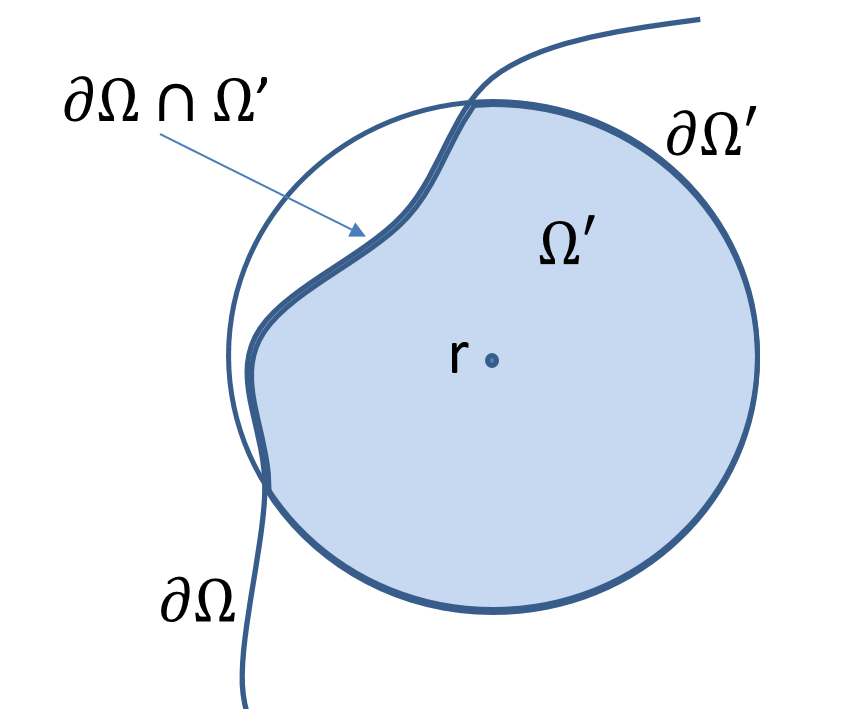
\includegraphics[width=0.30\linewidth]{Figures/3.Chapter/cont_kernel}
	\caption{Compact support kernel and domain boundary.}
	\label{fig:cont_kernel} 
\end{figure}
%
In this case the kernel zeroth-order momentum would not be one, deviating from the Dirac delta distribution and we would not be able to ensure first order consistency for the kernel approximation. Surface integrals in expressions \eqref{eq:grad_kernel_3} and \eqref{eq:grad_kernel_cond_2} would not disappear, leading to a loss of gradient information near the boundary and also order consistency. These problems meet various mitigation strategies at the discrete level, treated in section \ref{Subsec:discrete_interp}.

%%%%%%%%%%%%%%%%%%%%%%%%%%%%%%%%%%%%%%%%%%%%%%%%%%%%%%%%%%%%%%%%%%%%%%%%%%%%%%%%%
\subsection{Kernels}
\label{Subsec:Kernels}

In order to ensure the qualities of the continuous interpolation derived in Section \ref{Subsec:Interpolation}, the kernels must define a compact support region and have defined derivatives. A vast body of literature has been dedicated to the subject of kernels, their properties and their performance in the context of an \ac{SPH} simulation. Apparently similar kernels can produce very different results \citep{Monaghan-2005, Macia-2011,Violeau-2012}, and it is an ongoing task to formally identify and quantify the characteristics that lead to such differences. For the purpose of this thesis, only two kernels are described, a $5^{th}$ order class 2 Wendland \citep{Wendland-1995} and a cubic spline kernel. Both can be written as 

% 
\begin{equation} \label{eq:Kernel_general}
	W(\ve{r},h)=\frac{1}{h^d}\tilde{W}(q)
\end{equation}
%
where $h$ is the smoothing length and defines the scale of the compact support radius for kernel, $d$ is the dimensionality and $q=|\ve{r}|/h$ is a non-dimensional distance.

For the Wendland kernel, the $5^{th}$ order class 2 radial interpolation function was reformulated to have a $2h$ radius compact support

% 
\begin{equation} \label{eq:Kernel_wendeland}
	\tilde{W}(q)=\alpha_d\left\{ {\begin{array}{*{20}{c}}
  {(1-\frac{q}{2})^4(1+2q)} \\\\
  0 
\end{array}} \right.
\;\;\;\;\
\begin{array}{*{20}{c}}
  \text{for}\;\;\;{0 \leq q \leq 2} \\\\
  \text{for}\;\;\;{q > 2} 
\end{array}
\end{equation}
%
where $\alpha_d$ takes values $\alpha_2=7/4\pi$ and $\alpha_3=21/16\pi$. 

The cubic spline kernel can be defined as 

% 
\begin{equation} \label{eq:Kernel_cubic}
	\tilde{W}(q)=\alpha_d\left\{ {\begin{array}{*{20}{c}}
  {1-\frac{3}{2}q^2+\frac{3}{4}q^3} \\\\
  {\frac{1}{4}(2-q)^3} \\\\
  0 
\end{array}} \right.
\;\;\;\;\
\begin{array}{*{20}{c}}
  \text{for}\;\;\;{0 \leq q \leq 1} \\\\
  \text{for}\;\;\;{1 \leq q \leq 2} \\\\
  \text{for}\;\;\;{q > 2} 
\end{array}
\end{equation}
%
where $\alpha_2=10/7\pi$ and $\alpha_3=1/\pi$. Figure \ref{fig:kernel_wendland} plots the kernels and respective first derivatives.

%
\begin{figure}[ht!]
	\centering 
	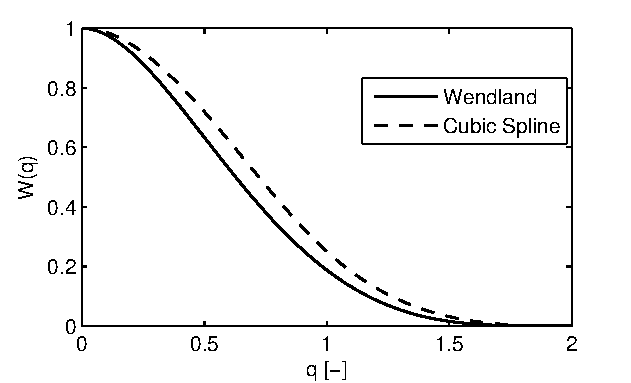
\includegraphics[width=0.49\linewidth]{Figures/3.Chapter/Kernels}
	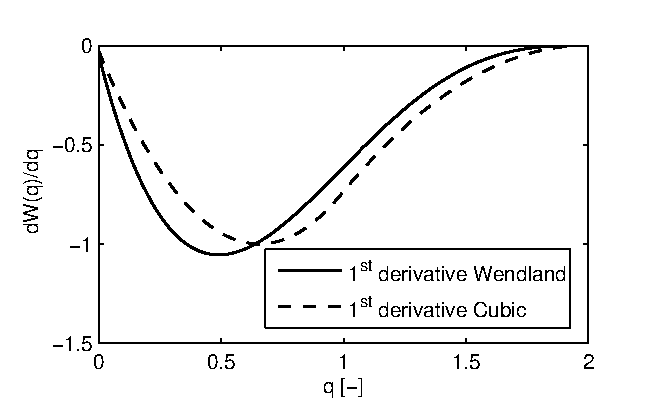
\includegraphics[width=0.49\linewidth]{Figures/3.Chapter/Kernels_deriv}
	\caption{Left - Wendland and Cubic spline kernels; Right - First derivatives.}
	\label{fig:kernel_wendland} 
\end{figure}
%
The kernels and the derivatives show very similar profiles, even tough they are one order apart. The cubic spline kernel is however known to cause tensile instability \cite{Monaghan-1999}, and requires corrections to definition \eqref{eq:Kernel_cubic}. According to \cite{Swegle-1995}, tensile instability seems to be directly related to the size of the region of the kernel where the second derivative is negative. Figure \ref{fig:kernel_wndland_d2} shows the second derivative of the considered kernels.

%
\begin{figure}[ht!]
	\centering 
	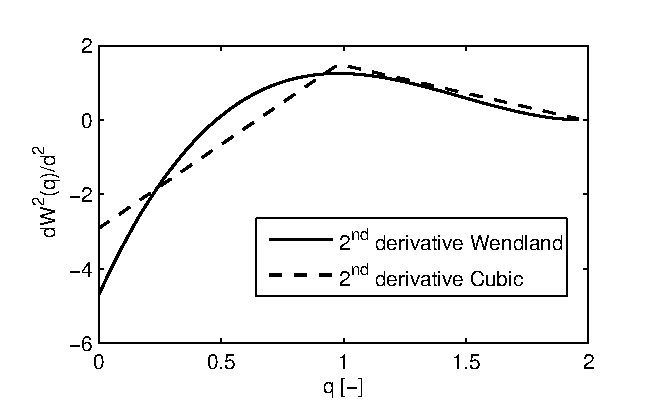
\includegraphics[width=0.49\linewidth]{Figures/3.Chapter/Kernels_2deriv}
	\caption{Second derivative of Wendland and Cubic spline kernels.}
	\label{fig:kernel_wndland_d2} 
\end{figure}
%
As can be noticed the size of these regions is similar, although the shape of the derivatives varies considerably. \cite{Macia-2011} performs an analysis of the performance of the Wendland kernel against a Gaussian kernel and finds that, even if apparently similar to the present comparison, the Wendland kernel out-performs other kernels considerably.


%%%%%%%%%%%%%%%%%%%%%%%%%%%%%%%%%%%%%%%%%%%%%%%%%%%%%%%%%%%%%%%%%%%%%%%%%%%%%%%%
\subsection{Discrete Interpolation}
\label{Subsec:discrete_interp}

As previously introduced, \ac{SPH} discretizes a continuous medium as a collection of Lagrangian interpolation nodes with mass. These points are called particles since they coincide with macroscopic material points that bear quantities such as velocity, density and position that change over time. Particle $i$ has a fixed mass of $m_i$, with volume $V_i$ and density $\rho_i$ related by

% 
\begin{equation} \label{eq:mass_volume_density}
V_i=\frac{m_i}{\rho_i}
\end{equation}
%
Assuming a reference density, a diameter $Dp$ can be set to compute the mass and reference volume of the particle.

In a strict Lagrangian framework, quantities of the particle will suffer a variation rate given by its Lagrangian derivative. For example, in the case of position and velocity

% 
\begin{equation} \label{eq:lagrang_posit}
\dot{\ve{r}}_i = \ve{v}_i = \frac{d\ve{r}_i}{dt}
\end{equation}
%
Expression \eqref{eq:lagrang_posit} contrasts with the Eulerian equivalent, since no advection terms are present, greatly simplifying the discretization.

The discretization of operators in \ac{SPH} is done by approximating the continuous integrals in section \ref{Subsec:Interpolation} by discrete summations. Employing a Riemann sum, one can write a scalar field as

% 
\begin{equation} \label{eq:discr_interp_1}
\left\langle {A} \right\rangle \left( {\ve{r}_i} \right) = \int_{\Omega '}  {A\left( {\ve{r}'} \right)\; W \left( {{\ve{r}_i} - {\ve{r}}', h} \right)d{{r}}'} \approx \sum_j{A_j V_j W(\ve{r}_{ij}, h)}
\end{equation}
%
The summation points are particle positions $\ve{r}_{j}$, where $A_j=A(\ve{r}_{j})$. $\ve{r}_{ij}$ represents $\ve{r}_{i}-\ve{r}_{j}$ and the volume of each $j$ particle accounts for the integration volume $d{\ve{r}}'$. Henceforth, without any loss of richness, the notation will be simplified: the subscripts $i$ and $j$ will tend to identify particles in the summation, $\ve{r}_{ij}$ will be used and it will be assumed that, dealing with a numerical approximation, the approximation notation will simply be represented by equality. The field is defined by the summation over all particles, but assuming compact support of the kernel this number is rendered finite. The sum is reduced to the particles inside the sphere of radius $\epsilon h$, as shown in Figure \ref{fig:kernel}

%
\begin{figure}[ht!]
	\centering 
	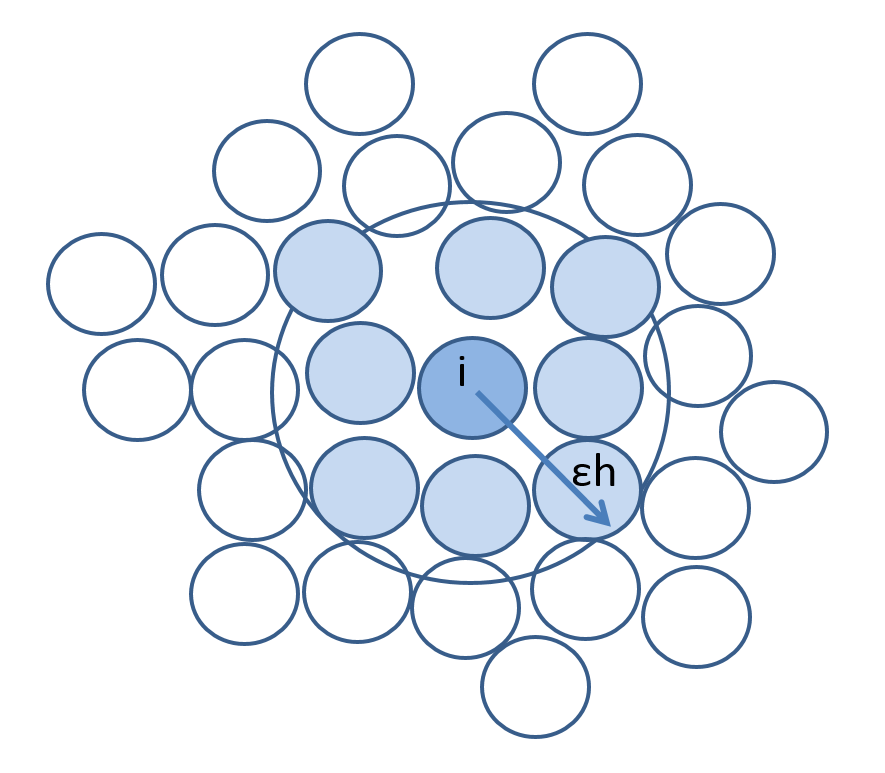
\includegraphics[width=0.40\linewidth]{Figures/3.Chapter/kernel}
	\caption{Summation extent for interpolation on particle $i$.}
	\label{fig:kernel} 
\end{figure}
%
In a 3 dimensions problem, the number of neighbors of a particle can range from a few tens to hundreds of points, summing an important disadvantage \ac{SPH} presents when compared with traditional, mesh-based methods: large computational cost.

Applying the discrete operator \eqref{eq:discr_interp_1} to vectorial quantities and notion \eqref{eq:grad_kernel_4} to differential operators we can write

% 
\begin{equation} \label{eq:discr_interp_2}
\begin{split}
A_i = \sum_j{A_j V_j W(\ve{r}_{ij}, h)} \\
\nabla {A}_i = \sum_j{A_j V_j \nabla W(\ve{r}_{ij}, h)} \\
\ve{A}_i = \sum_j{\ve{A}_j V_j W(\ve{r}_{ij}, h)} \\
\ve{\nabla} \cdot \ve{A}_i = \sum_j{ V_j \ve{A}_j \cdot \ve{\nabla} W(\ve{r}_{ij}, h)} 
\end{split}
\end{equation}
%

It should be noted that these expressions, although representing an exact derivative of the approximate function (considering no truncation effects on the kernel sampling), are written in a form that leads to a non zero derivative for a constant field. To ensure that gradients respect these properties one can write

% 
\begin{equation} \label{eq:discr_interp_3}
\nabla {A} = \frac{1}{\Phi}\left( \nabla(\Phi A)- A\nabla\Phi \right)
\end{equation}
%
where $\Phi$ is a differentiable function. In \ac{SPH} form

% 
\begin{equation} \label{eq:discr_interp_4}
\nabla {A}_i = \frac{1}{\Phi_i} \sum_j{\Phi_j V_j(A_j-A_i) \nabla W(\ve{r}_{ij}, h)}
\end{equation}
%
Equation \eqref{eq:discr_interp_4} returns a zero gradient for a constant field.  

Second derivatives can be estimated by differentiating an \ac{SPH} interpolant (Equation \eqref{eq:discr_interp_1}) twice:

% 
\begin{equation} \label{eq:2nd_der_sph_I}
\nabla^2 {A}_i  = \sum_j{A_j V_j \nabla^2 W(\ve{r}_{ij}, h)} 
\end{equation}
%
This expression, however elegant, presents a series of problems: i) it is very sensitive to particle disorder; ii) it is trivial to build a kernel whose second derivative changes sign on its defined region, possibly changing the sign of the second derivative independently of the behavior of the quantity, among other issues, properly explored by \cite{Brookshaw-1985, Monaghan-2005}. A more useful approach was proposed by \cite{Cleary-1996} and \cite{Morris-1997}

% 
\begin{equation} \label{eq:2nd_der_sph_II}
\nabla^2 {A}_i = \sum_j{A_j V_j \frac{\ve{r}_{ij}\cdot W(\ve{r}_{ij}, h)}{||\ve{r}_{ij}||^2}}
\end{equation}
%
This represents a hybrid combination of a finite difference derivative and a \ac{SPH} derivative. It has the advantage of bypassing the issues raised by taking a direct second derivative of the kernel function, at the expense of not fully conserving angular momentum \citep{Monaghan-2006}.

















